% !TeX root = ../main-english.tex
% !TeX spellcheck = en-US
% !TeX encoding = utf8
% -*- coding:utf-8 mod:LaTeX -*-

%This smart spell only works if no changes have been made to the chapter
%using the options proposed in preambel/chapterheads.tex.
\setchapterpreamble[u]{%
	\dictum[Carole Goble]{Better Software, Better Research}
}

%\chapter{Improving scientific practice through software usability: The DataLad Handbook}
\chapter{Improving scientific practice through software usability}
\label{chap:k2}




This next chapter details how a documentation project for DataLad increased software quality, software popularity and enabled users to tackle complex \gls{rdm} use cases.
It refers to our original publication \citep{wagner2020datalad}.


\section{Scientific software}

Scientific software, often also referred to as research software, is an integral part of research in science, engineering, and humanities.
It can broadly be defined as software used for scientific purposes.
As software requirements for scientific use cases can be specialized, the developers of research software often overlap with the community of scientists that uses the software, and over the past decade, the term ``Research Software Engineer'' has been established to describe researchers that dedicate parts of their scientific work to creating and maintaining software \citep{hettrickRSE}



The United Kingdom's Engineering and Physical Sciences Research Council describes software as a ``critical infrastructure that underpins cutting edge science and engineering research'' (CITATION) % https://www.ukri.org/what-we-offer/browse-our-areas-of-investment-and-support/research-infrastructure-theme/

More recently, research software has been gaining academic credit it has long lacked.
It is recognized as academic output in the San Francisco Declaration on Research Assessment (DORA; \href{https://sfdora.org/}{sfdora.org}), and the Agreement on Reforming Research Assessment (CoARA; \href{https://coara.eu}{coara.eu}), both of which have been signed by thousands of academic institutions worldwide. The \gls{grf}, the largest funding institution for the sciences and humanities and research in Germany, counts software a ``scientific result'' in their evaluation of academic CVs.
Academic journals, such as the Journal of Open Source Software (\href{https://joss.theoj.org/}{joss.theoj.org/}), and article types, such as ``Nature Toolbox'' (\href{https://www.nature.com/nature/articles?type=toolbox}{www.nature.com/nature/articles?type=toolbox}), have been created to support the scholarly publication and reuse of research software.
And calls for proposals to improve the quality, usability or longevity of research software have been put forward by major funders, for example in Germany \citep{dfgrs}, the United Kingdom \citep{ukri}, or the United States \citep{nih}.



The largest funding institution for the sciences and humanities and research in Germany, the \gls{grf}, states that access to data and software are of comparable importance to science as access to publications \citep{dfg}

The DFG put forward several timely recommendations: Research software should be open source \citep{dfg}


\subsection{Documentation deficits of scientific software and their consequences}

Even if state-of-the art software tools that could improve scientific practice exist, their mere existence is insufficient to ensure uptake and use according to best practices.
To improve scientific practice, software tools need to enable and empower their users through usability and documentation.
This makes documentation a major factor in the success of scientific software, and an integral part of the software development process.
% what is documentation, provide definitions/delineations
Documentation is information about a software.
It fulfills different roles, depending on its target audience, and the literature distinguishes several different types of documentation.
\citet{Parnas2011} categorizes documentation either as a \textit{tutorial} or as a \textit{reference work}.
Both kinds are needed for different audiences: Whereas experienced users and contributors need reference documents to guide further development, such as the elements of an \gls{api}, new users and contributors need a basic understanding of the software tool and its intended use cases.
Commonly distinguished are also \textit{technical} and \textit{user} documentation: The former contains information for developers and users by describing features, maintenance information, or design choices.
The latter targets end users of a software product with accessible explanations how to install a tool, use its features, or step-by-step instructions (CITATION NEEDED). % https://medium.com/@kesiparker/technical-documentation-vs-user-documentation-ff68e7de1985
User documentation also matches the concept of \textit{task-based} documentation, which is broken down into the activities that users will go through as they work, starting with basic tasks and continuing with more advanced tasks that become possible as users continue to work. (CITATION NEEDED) %https://www.linux-magazine.com/Online/Blogs/Off-the-Beat-Bruce-Byfield-s-Blog/Why-projects-need-task-based-documentation

% maybe Design/Architectural docs

Scientific software often lacks comprehensive documentation \citep{segal2007some} \citep{pawlik2012documentation}.
Commonly reported reasons for this are a lack of funding, incentives, and interest by software developers \citep{pawlik2012documentation}.

% consequences

Yet although it is commonly regarded as separate from the actual piece of software, software documentation is heavily tied to the quality of a software tool and the software development process.
A lack of documentation hinders knowledge transfer both among users and developers, impedes maintenance, and creates a steep learning curve for new users and new developers alike \citep{theunissen}.
\citet{Parnas2011} describes a vicious circle that sets in when the quality of software documentation is poor:
``Reduced [documentation] quality leads to reduced [software] usage, [r]educed [software] usage leads to reductions in both resources and motivation, [r]educed resources and motivation degrade [software] quality further''
% maybe workflows that break, workflow testing


\section{Documentation in the DataLad project}

Since the first release (0.0.1, March 2015), DataLad had technical documentation with a design overview and a reference documentation.
Any amount of documentation is better than no documentation at all.
However, documentation can still be insufficient if it does not meet the needs of the target audience.
Solely technical or reference documentation, for example, can be suboptimal for novices: It may be incomplete, narrowly focused on individual commands, or assume existing knowledge readers lack (Segal, 2007; Pawlik et al., 2015), and can thereby discourage potential users or inhibit the adoption of valuable tools.\\
Even though technical documentation is useful for developers, a central target audience for documentation of the DataLad ecosystem are scientists.
While experts in their respective domains and methodologies, scientists may not have domain-agnostic technical skills.
Task sets such as those required in \gls{rdm} require a broad set of technical skills, however, which is \citep{grisham2016proposed}.
Research curricula seldom teach computing ecosystem literacy.
In fact, even computer science curricula often miss critical topics about the computing ecosystem.
At the \gls{MIT}, this lack famously resulted in the internationally popular, self-organized class ``The missing semester of CS education'' (\href{https://missing.csail.mit.edu/about/}{missing.csail.mit.edu}).
In addition, the high usability of modern computers' and applications' front ends spares users the need to develop the same level of familiarity with their computers than previous generations of computer users had \citep{mehlenbacher2003documentation}. \\
Research suggests, too, that scientists' needs for documentation go beyond reference manuals.
In an analysis of user questions in support forums of scientific software packages, \citet{swarts2019open} found that the focus in 80\% of inquiries was on operations and tasks, such as a required sequence of operations to achieve a specific goal.
In breaking down user questions by purpose, \citet{swarts2019open} further found that users were most interested in a description of operations or tasks, followed by insights about the reasons behind the action.
And in separating documentation types into ``feature-based'' (closer related to the concept of reference documentation) or ``task-based'',  \citet{swarts2019open} reports twice as many questions seeking explanations in software with feature-based compared to task-based documentation.
This hints at a disconnect between knowing \textit{how} something should be done and \textit{why} it should be done this way.
Overall, it highlights that users of scientific software show a clear need beyond the documentation of individual commands, but seek to understand general usage principles and master complex combinations of features to achieve specified goals.
This type of empowerment is what the DataLad handbook project aimed to achieve.


Only rarely does a consumer tool involve a terminal instead of a \gls{gui}, and typical applications perform a complete suite of tasks such that users do not need to combine several tools to accomplish one goal (CITATION NEEDED).
However, powerful scientific tools are often command-line-based (e.g., EXAMPLES), and complex task sets such as those required in \gls{rdm} require a broad set of technical skills \citep{grisham2016proposed}.
DataLad, too, is primarily developed as a command line tool.

\pagebreak

\subsection{The DataLad Handbook: A user-focused and workflow-based addition to standard software documentation}

The initial idea to the DataLad Handbook arose at the 2019 Meeting of the \gls{ohbm}, during the Symposium ``From Open Science to Science: Shifting the status quo in data sharing, software, and publishing''.
Gregory Kiar's presentation ``Technology and Platforms Enabling Reproducible and Open Publishing'' included a recommendation and warning about DataLad: While it would be a powerful tool capable of solving many challenges, users will face difficulties learning which features existed and how they could use them \citep{kiar}.
Motivated by this expressed need of the scientific community for additional guidance, the DataLad Handbook project was set out with the following goals:



A user-driven alternative to reference documentation by software developers, ``Documentation Crowdsourcing'', has been successfully employed by the NumPy project \citep{pawlik2014crowdsourcing}.
Extending this concept beyond documentation, we have created the DataLad handbook (\href{http://handbook.datalad.org}{handbook.datalad.org}) as a free and open-source, user-driven and -focused narrative tutorial.



Usability adherence

Timeline:
The DataLad Handbook has been under continuous development for more than three years, averaging two releases per year.
As of May 2023, a total of 53 contributors provided input in the form of content, bug fixes, or infrastructure improvements.
During December 2022 and July 2023, the DataLad Handbook averaged 30000 total page views per 30 days.


\begin{figure}
	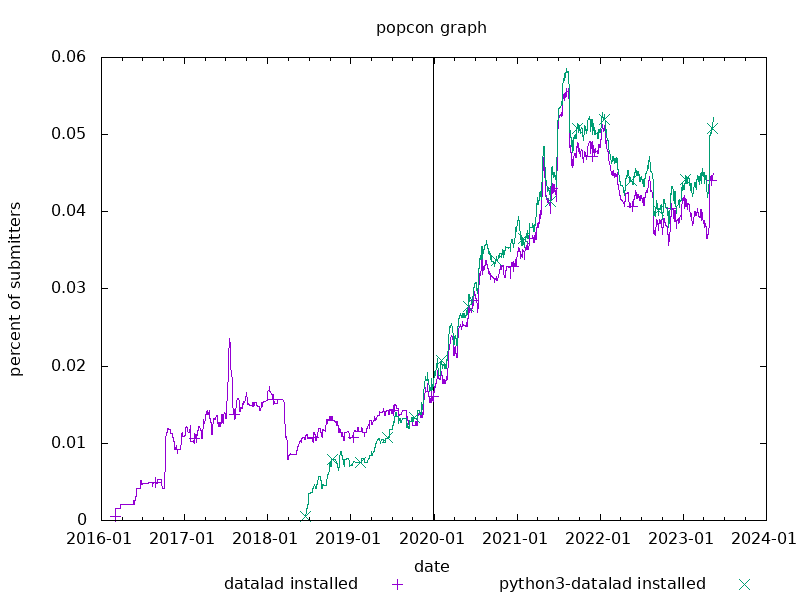
\includegraphics[width=\textwidth]{popcon-datalad.png}
	\caption{d}
	\label{fig:popcon}
\end{figure}

\pagebreak

